% Created 2017-01-19 jeu. 15:02
\documentclass[11pt]{article}
\usepackage[utf8]{inputenc}
\usepackage[T1]{fontenc}
\usepackage{fixltx2e}
\usepackage{graphicx}
\usepackage{grffile}
\usepackage{longtable}
\usepackage{wrapfig}
\usepackage{rotating}
\usepackage[normalem]{ulem}
\usepackage{amsmath}
\usepackage{textcomp}
\usepackage{amssymb}
\usepackage{capt-of}
\usepackage{hyperref}
\author{Maxime Chevalier}
\date{\today}
\title{Laboratory Notebook for a Multi-Threaded Version of Quicksort}
\hypersetup{
 pdfauthor={Maxime Chevalier},
 pdftitle={Laboratory Notebook for a Multi-Threaded Version of Quicksort},
 pdfkeywords={},
 pdfsubject={},
 pdfcreator={Emacs 24.5.1 (Org mode 8.3.3)}, 
 pdflang={Frenchb}}
\begin{document}

\maketitle
\tableofcontents


\section{Indroduction}
\label{sec:orgheadline1}
Ce journal est le compte rendu d'un élève de RICM4 à Grenoble.
\section{Caractéristiques de la machine}
\label{sec:orgheadline5}
\subsection{Version du système d'exploitation}
\label{sec:orgheadline2}
\begin{verbatim}
uname -a;
\end{verbatim}

\begin{verbatim}
Linux chevamax-Satellite-Pro-R50-B 4.4.0-21-generic #37-Ubuntu SMP Mon Apr 18 18:33:37 UTC 2016 x86_64 x86_64 x86_64 GNU/Linux
\end{verbatim}

\subsection{CPU}
\label{sec:orgheadline3}
\begin{verbatim}
lscpu;
\end{verbatim}

\begin{center}
\begin{tabular}{lllllllllllllllllllllllllllllllllllllllllllllllllllllllllllllllllllllllllllllllllllllllllll}
Architecture: & x86\(_{\text{64}}\) &  &  &  &  &  &  &  &  &  &  &  &  &  &  &  &  &  &  &  &  &  &  &  &  &  &  &  &  &  &  &  &  &  &  &  &  &  &  &  &  &  &  &  &  &  &  &  &  &  &  &  &  &  &  &  &  &  &  &  &  &  &  &  &  &  &  &  &  &  &  &  &  &  &  &  &  &  &  &  &  &  &  &  &  &  &  &  &  & \\
Mode(s) & opératoire(s) & des & processeurs :32-bit, & 64-bit &  &  &  &  &  &  &  &  &  &  &  &  &  &  &  &  &  &  &  &  &  &  &  &  &  &  &  &  &  &  &  &  &  &  &  &  &  &  &  &  &  &  &  &  &  &  &  &  &  &  &  &  &  &  &  &  &  &  &  &  &  &  &  &  &  &  &  &  &  &  &  &  &  &  &  &  &  &  &  &  &  &  &  &  &  & \\
Byte & Order: & Little & Endian &  &  &  &  &  &  &  &  &  &  &  &  &  &  &  &  &  &  &  &  &  &  &  &  &  &  &  &  &  &  &  &  &  &  &  &  &  &  &  &  &  &  &  &  &  &  &  &  &  &  &  &  &  &  &  &  &  &  &  &  &  &  &  &  &  &  &  &  &  &  &  &  &  &  &  &  &  &  &  &  &  &  &  &  &  &  & \\
CPU(s): & 4 &  &  &  &  &  &  &  &  &  &  &  &  &  &  &  &  &  &  &  &  &  &  &  &  &  &  &  &  &  &  &  &  &  &  &  &  &  &  &  &  &  &  &  &  &  &  &  &  &  &  &  &  &  &  &  &  &  &  &  &  &  &  &  &  &  &  &  &  &  &  &  &  &  &  &  &  &  &  &  &  &  &  &  &  &  &  &  &  & \\
On-line & CPU(s) & list: & 0-3 &  &  &  &  &  &  &  &  &  &  &  &  &  &  &  &  &  &  &  &  &  &  &  &  &  &  &  &  &  &  &  &  &  &  &  &  &  &  &  &  &  &  &  &  &  &  &  &  &  &  &  &  &  &  &  &  &  &  &  &  &  &  &  &  &  &  &  &  &  &  &  &  &  &  &  &  &  &  &  &  &  &  &  &  &  &  & \\
Thread(s) & par & cœur : & 2 &  &  &  &  &  &  &  &  &  &  &  &  &  &  &  &  &  &  &  &  &  &  &  &  &  &  &  &  &  &  &  &  &  &  &  &  &  &  &  &  &  &  &  &  &  &  &  &  &  &  &  &  &  &  &  &  &  &  &  &  &  &  &  &  &  &  &  &  &  &  &  &  &  &  &  &  &  &  &  &  &  &  &  &  &  &  & \\
Cœur(s) & par & socket : & 2 &  &  &  &  &  &  &  &  &  &  &  &  &  &  &  &  &  &  &  &  &  &  &  &  &  &  &  &  &  &  &  &  &  &  &  &  &  &  &  &  &  &  &  &  &  &  &  &  &  &  &  &  &  &  &  &  &  &  &  &  &  &  &  &  &  &  &  &  &  &  &  &  &  &  &  &  &  &  &  &  &  &  &  &  &  &  & \\
Socket(s): & 1 &  &  &  &  &  &  &  &  &  &  &  &  &  &  &  &  &  &  &  &  &  &  &  &  &  &  &  &  &  &  &  &  &  &  &  &  &  &  &  &  &  &  &  &  &  &  &  &  &  &  &  &  &  &  &  &  &  &  &  &  &  &  &  &  &  &  &  &  &  &  &  &  &  &  &  &  &  &  &  &  &  &  &  &  &  &  &  &  & \\
Nœud(s) & NUMA : & 1 &  &  &  &  &  &  &  &  &  &  &  &  &  &  &  &  &  &  &  &  &  &  &  &  &  &  &  &  &  &  &  &  &  &  &  &  &  &  &  &  &  &  &  &  &  &  &  &  &  &  &  &  &  &  &  &  &  &  &  &  &  &  &  &  &  &  &  &  &  &  &  &  &  &  &  &  &  &  &  &  &  &  &  &  &  &  &  & \\
Identifiant & constructeur :GenuineIntel &  &  &  &  &  &  &  &  &  &  &  &  &  &  &  &  &  &  &  &  &  &  &  &  &  &  &  &  &  &  &  &  &  &  &  &  &  &  &  &  &  &  &  &  &  &  &  &  &  &  &  &  &  &  &  &  &  &  &  &  &  &  &  &  &  &  &  &  &  &  &  &  &  &  &  &  &  &  &  &  &  &  &  &  &  &  &  &  & \\
Famille & de & processeur :6 &  &  &  &  &  &  &  &  &  &  &  &  &  &  &  &  &  &  &  &  &  &  &  &  &  &  &  &  &  &  &  &  &  &  &  &  &  &  &  &  &  &  &  &  &  &  &  &  &  &  &  &  &  &  &  &  &  &  &  &  &  &  &  &  &  &  &  &  &  &  &  &  &  &  &  &  &  &  &  &  &  &  &  &  &  &  &  & \\
Modèle : & 69 &  &  &  &  &  &  &  &  &  &  &  &  &  &  &  &  &  &  &  &  &  &  &  &  &  &  &  &  &  &  &  &  &  &  &  &  &  &  &  &  &  &  &  &  &  &  &  &  &  &  &  &  &  &  &  &  &  &  &  &  &  &  &  &  &  &  &  &  &  &  &  &  &  &  &  &  &  &  &  &  &  &  &  &  &  &  &  &  & \\
Model & name: & Intel(R) & Core(TM) & i5-4210U & CPU & @ & 1.70GHz &  &  &  &  &  &  &  &  &  &  &  &  &  &  &  &  &  &  &  &  &  &  &  &  &  &  &  &  &  &  &  &  &  &  &  &  &  &  &  &  &  &  &  &  &  &  &  &  &  &  &  &  &  &  &  &  &  &  &  &  &  &  &  &  &  &  &  &  &  &  &  &  &  &  &  &  &  &  &  &  &  &  & \\
Révision : & 1 &  &  &  &  &  &  &  &  &  &  &  &  &  &  &  &  &  &  &  &  &  &  &  &  &  &  &  &  &  &  &  &  &  &  &  &  &  &  &  &  &  &  &  &  &  &  &  &  &  &  &  &  &  &  &  &  &  &  &  &  &  &  &  &  &  &  &  &  &  &  &  &  &  &  &  &  &  &  &  &  &  &  &  &  &  &  &  &  & \\
Vitesse & du & processeur & en & MHz :997.875 &  &  &  &  &  &  &  &  &  &  &  &  &  &  &  &  &  &  &  &  &  &  &  &  &  &  &  &  &  &  &  &  &  &  &  &  &  &  &  &  &  &  &  &  &  &  &  &  &  &  &  &  &  &  &  &  &  &  &  &  &  &  &  &  &  &  &  &  &  &  &  &  &  &  &  &  &  &  &  &  &  &  &  &  &  & \\
CPU & max & MHz: & 2700,0000 &  &  &  &  &  &  &  &  &  &  &  &  &  &  &  &  &  &  &  &  &  &  &  &  &  &  &  &  &  &  &  &  &  &  &  &  &  &  &  &  &  &  &  &  &  &  &  &  &  &  &  &  &  &  &  &  &  &  &  &  &  &  &  &  &  &  &  &  &  &  &  &  &  &  &  &  &  &  &  &  &  &  &  &  &  &  & \\
CPU & min & MHz: & 800,0000 &  &  &  &  &  &  &  &  &  &  &  &  &  &  &  &  &  &  &  &  &  &  &  &  &  &  &  &  &  &  &  &  &  &  &  &  &  &  &  &  &  &  &  &  &  &  &  &  &  &  &  &  &  &  &  &  &  &  &  &  &  &  &  &  &  &  &  &  &  &  &  &  &  &  &  &  &  &  &  &  &  &  &  &  &  &  & \\
BogoMIPS: & 4788.54 &  &  &  &  &  &  &  &  &  &  &  &  &  &  &  &  &  &  &  &  &  &  &  &  &  &  &  &  &  &  &  &  &  &  &  &  &  &  &  &  &  &  &  &  &  &  &  &  &  &  &  &  &  &  &  &  &  &  &  &  &  &  &  &  &  &  &  &  &  &  &  &  &  &  &  &  &  &  &  &  &  &  &  &  &  &  &  &  & \\
Virtualisation : & VT-x &  &  &  &  &  &  &  &  &  &  &  &  &  &  &  &  &  &  &  &  &  &  &  &  &  &  &  &  &  &  &  &  &  &  &  &  &  &  &  &  &  &  &  &  &  &  &  &  &  &  &  &  &  &  &  &  &  &  &  &  &  &  &  &  &  &  &  &  &  &  &  &  &  &  &  &  &  &  &  &  &  &  &  &  &  &  &  &  & \\
Cache & L1d : & 32K &  &  &  &  &  &  &  &  &  &  &  &  &  &  &  &  &  &  &  &  &  &  &  &  &  &  &  &  &  &  &  &  &  &  &  &  &  &  &  &  &  &  &  &  &  &  &  &  &  &  &  &  &  &  &  &  &  &  &  &  &  &  &  &  &  &  &  &  &  &  &  &  &  &  &  &  &  &  &  &  &  &  &  &  &  &  &  & \\
Cache & L1i : & 32K &  &  &  &  &  &  &  &  &  &  &  &  &  &  &  &  &  &  &  &  &  &  &  &  &  &  &  &  &  &  &  &  &  &  &  &  &  &  &  &  &  &  &  &  &  &  &  &  &  &  &  &  &  &  &  &  &  &  &  &  &  &  &  &  &  &  &  &  &  &  &  &  &  &  &  &  &  &  &  &  &  &  &  &  &  &  &  & \\
Cache & L2 : & 256K &  &  &  &  &  &  &  &  &  &  &  &  &  &  &  &  &  &  &  &  &  &  &  &  &  &  &  &  &  &  &  &  &  &  &  &  &  &  &  &  &  &  &  &  &  &  &  &  &  &  &  &  &  &  &  &  &  &  &  &  &  &  &  &  &  &  &  &  &  &  &  &  &  &  &  &  &  &  &  &  &  &  &  &  &  &  &  & \\
Cache & L3 : & 3072K &  &  &  &  &  &  &  &  &  &  &  &  &  &  &  &  &  &  &  &  &  &  &  &  &  &  &  &  &  &  &  &  &  &  &  &  &  &  &  &  &  &  &  &  &  &  &  &  &  &  &  &  &  &  &  &  &  &  &  &  &  &  &  &  &  &  &  &  &  &  &  &  &  &  &  &  &  &  &  &  &  &  &  &  &  &  &  & \\
NUMA & node0 & CPU(s): & 0-3 &  &  &  &  &  &  &  &  &  &  &  &  &  &  &  &  &  &  &  &  &  &  &  &  &  &  &  &  &  &  &  &  &  &  &  &  &  &  &  &  &  &  &  &  &  &  &  &  &  &  &  &  &  &  &  &  &  &  &  &  &  &  &  &  &  &  &  &  &  &  &  &  &  &  &  &  &  &  &  &  &  &  &  &  &  &  & \\
Flags: & fpu & vme & de & pse & tsc & msr & pae & mce & cx8 & apic & sep & mtrr & pge & mca & cmov & pat & pse36 & clflush & dts & acpi & mmx & fxsr & sse & sse2 & ss & ht & tm & pbe & syscall & nx & pdpe1gb & rdtscp & lm & constant\(_{\text{tsc}}\) & arch\(_{\text{perfmon}}\) & pebs & bts & rep\(_{\text{good}}\) & nopl & xtopology & nonstop\(_{\text{tsc}}\) & aperfmperf & eagerfpu & pni & pclmulqdq & dtes64 & monitor & ds\(_{\text{cpl}}\) & vmx & est & tm2 & ssse3 & sdbg & fma & cx16 & xtpr & pdcm & pcid & sse4\(_{\text{1}}\) & sse4\(_{\text{2}}\) & movbe & popcnt & tsc\(_{\text{deadline}}_{\text{timer}}\) & aes & xsave & avx & f16c & rdrand & lahf\(_{\text{lm}}\) & abm & epb & tpr\(_{\text{shadow}}\) & vnmi & flexpriority & ept & vpid & fsgsbase & tsc\(_{\text{adjust}}\) & bmi1 & avx2 & smep & bmi2 & erms & invpcid & xsaveopt & dtherm & ida & arat & pln & pts\\
\end{tabular}
\end{center}

\subsection{RAM}
\label{sec:orgheadline4}
\begin{verbatim}
free -m;
\end{verbatim}

\begin{center}
\begin{tabular}{llrrrrr}
total & utilisé & libre & partagé & tamp/cache & disponible & \\
Mem: & 7898 & 1702 & 1133 & 366 & 5062 & 5751\\
Partition & d'échange: & 7996 & 0 & 7996 &  & \\
\end{tabular}
\end{center}

\section{Test 1}
\label{sec:orgheadline9}
Réexecution du code sur ma machine 

\begin{verbatim}
"exports both"body
\end{verbatim}

\subsection{Analyse des résultats}
\label{sec:orgheadline6}
On voit ici que les résultats sont complétement différents (et même
plutot incohérents\ldots{}). A se demander si la machine utilise ses
différents coeurs!

\subsection{Retestons en branchant !}
\label{sec:orgheadline7}

\begin{verbatim}
"exports both"body
\end{verbatim}

\subsection{Analyse}
\label{sec:orgheadline8}
C'est pas mieux \ldots{}

\section{Test 2}
\label{sec:orgheadline10}
Nous allons garder les mêmes valeurs en mélangeant l'ordre d'execution


\begin{verbatim}
OUTPUT_DIRECTORY=data/`hostname`_`date +%F`
mkdir -p $OUTPUT_DIRECTORY
OUTPUT_FILE=$OUTPUT_DIRECTORY/measurements_`date +%R`.txt

touch $OUTPUT_FILE

for rep in `seq 1 5`; do
	for i in 100 1000 10000 100000 1000000; do
		echo "Size: $i" >> $OUTPUT_FILE;
		./src/parallelQuicksort $i >> $OUTPUT_FILE;
	done
done
\end{verbatim}

\begin{verbatim}
FILENAME="data/chevamax-Satellite-Pro-R50-B_2017-01-19/measurements_14:57"
perl scripts/csv_quicksort_extractor2.pl < "$FILENAME.txt" > "${FILENAME}_wide.csv"
echo "
  set terminal png size 600,400 
  set output '${FILENAME}_wide.png'
  set datafile separator ','
  set key autotitle columnhead
  plot '${FILENAME}_wide.csv' using 1:2 with linespoints, '' using 1:3 with linespoints, '' using 1:4 with linespoints
" | gnuplot
echo [[file:${FILENAME}_wide.png]]
\end{verbatim}

\section{Test 3}
\label{sec:orgheadline11}
Dans ce premier test nous allons affiner la courbe en faisant des tests
sur des tableaux de taille 10, 50, 100, 500, 1000, 5000, 10000, 50000,
100000, 500000 et 1000000.

Nous allons effectuer le test 10 fois pour chaque valeur.

\begin{verbatim}
::::::::::::::
scripts/run_benchmarking.sh
::::::::::::::

OUTPUT_DIRECTORY=data/`hostname`_`date +%F`
mkdir -p $OUTPUT_DIRECTORY
OUTPUT_FILE=$OUTPUT_DIRECTORY/measurements_`date +%R`.txt

touch $OUTPUT_FILE
for i in 10 50 100 500 1000 5000 10000 50000 100000 500000 1000000; do
    for rep in `seq 1 10`; do
        echo "Size: $i" >> $OUTPUT_FILE;
        ./src/parallelQuicksort $i >> $OUTPUT_FILE;
    done ;
done
\end{verbatim}

Pour transformer le fichier texte en fichier on utilise le script
fourni et la commande :

\begin{verbatim}
FILENAME="data/chevamax-Satellite-Pro-R50-B_2017-01-18/measurements_19:40"
perl scripts/csv_quicksort_extractor2.pl < "$FILENAME.txt" > "${FILENAME}_wide.csv"
echo "
  set terminal png size 600,400 
  set output '${FILENAME}_wide.png'
  set datafile separator ','
  set key autotitle columnhead
  plot '${FILENAME}_wide.csv' using 1:2 with linespoints, '' using 1:3 with linespoints, '' using 1:4 with linespoints
" | gnuplot
echo [[file:${FILENAME}_wide.png]]
\end{verbatim}

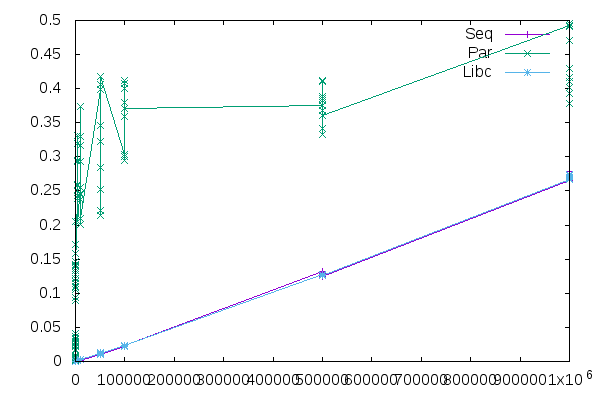
\includegraphics[width=.9\linewidth]{data/chevamax-Satellite-Pro-R50-B_2017-01-18/measurements_19:40_wide.png}
\end{document}